\documentclass[spanish, 12pt]{book}
\usepackage[T1]{fontenc}
\usepackage[utf8]{inputenc}
\usepackage{lmodern}
\usepackage[a4paper]{geometry}
\usepackage[spanish]{babel}
\usepackage{hyperref}
\usepackage{csquotes}

% Bibliorafía
\usepackage[style=apa,sorting=nyt,backend=biber]{biblatex}
\DeclareLanguageMapping{spanish}{spanish-apa}
\bibliography{references}
%

%\usepackage[]{parskip}
\usepackage{multicol}
\usepackage{multirow}
\usepackage[x11names,table]{xcolor} 
\usepackage{floatrow}
\usepackage{graphicx}
\usepackage{amsmath, latexsym, amsfonts, amssymb} 
\usepackage{booktabs}
\usepackage{url}
%\usepackage{float}
\usepackage[shortlabels]{enumitem}
\usepackage{tikz}
\usepackage{floatrow}
\usepackage[bf,labelsep=period]{caption}
\captionsetup{justification = centering}
\renewcommand{\baselinestretch}{1.5} % interlineado
\usepackage[bottom]{footmisc}

\usepackage{mathtools}
\usepackage{optidef}

% Se añadió ahora para las referencias
\usepackage{cleveref}
% Comentarios
%\usepackage{comment}
%\usepackage{todonotes}
%\usepackage{easyReview}
%

% Python
\usepackage{listings}
%\usepackage{listingsutf8}
\usepackage{color}


% Redefinir el nombre del listing
\renewcommand{\lstlistingname}{Ejemplo} % <--- AQUÍ EL CAMBIO

\definecolor{mygreen}{rgb}{0,0.6,0}
\definecolor{mygray}{rgb}{0.5,0.5,0.5}
\definecolor{mymauve}{rgb}{0.58,0,0.82}
\definecolor{myred}{rgb}{0.58,0,0}


\lstset{ 
	backgroundcolor=\color{white},
	basicstyle=\footnotesize,
	breakatwhitespace=false,  
	breaklines=true,         
	captionpos=b,            
	commentstyle=\color{mygray},   
	deletekeywords={...},   
	escapeinside={\%*}{*)},         
	extendedchars=true,             
	firstnumber=1,               
	frame=,	     
%	identifierstyle=\color{blue},             
	keepspaces=true,                
	keywordstyle=\bfseries\color{mygreen},      
	language=Python,                
	morekeywords={*, ..., Var, AbstractModel, Param, Set, Obective, Constraint, Complementarity},            
	numbers=none,   % Posición de los números de línea (none, left, right).                 
	numbersep=5pt,                   
	numberstyle=\tiny\color{mygray},
	rulecolor=\color{blue},        
	showspaces=false,                
	showstringspaces=false,          
	showtabs=false,                
	stepnumber=1,                    
	stringstyle=\color{myred},     
	tabsize=2,	                  
	title=\lstname                  
}
%

\newcommand{\R}{\mathbb{R}} 
\newcommand{\N}{\mathbb{N}} 
\newcommand{\Z}{\mathbb{Z}} 
\newcommand{\Lagr}{\mathcal{L}}
% Agregar argmin
% En el preámbulo del documento
\usepackage{amsmath}
\DeclareMathOperator*{\argmin}{argmin} % Define el operador argmin

% Dar formato codigo de julia
\usepackage{listings}
\usepackage{xcolor}

% Configuración para código Julia
\usepackage{listings}
\usepackage{xcolor}
\usepackage{cmap} % Mejora la capacidad de copiar/pegar
\usepackage[T1]{fontenc}
% Definición manual del lenguaje Julia
\lstdefinelanguage{Julia}%
{
  keywords={abstract,break,case,catch,const,continue,do,else,elseif,end,%
    export,false,for,function,if,immutable,import,importall,in,let,macro,%
    module,mutable,null,primitive,quote,return,struct,switch,true,try,type,%
    using,while},%
  sensitive=true,%
  alsoother={$},%
  morecomment=[l]\#,%
  morecomment=[n]{\#=}{=\#},%
  morestring=[s]{"}{"},%
  morestring=[m]{'}{'},%
}[keywords,comments,strings]

% Configuración del estilo
\lstdefinestyle{julia-style}{
    language=Julia,
    basicstyle=\ttfamily\small,
    breaklines=true,
    showstringspaces=false,
    commentstyle=\color{green!60!black},
    keywordstyle=\color{blue},
    stringstyle=\color{red},
    frame=single,
    numbers=left,
    numberstyle=\tiny\color{gray},
    backgroundcolor=\color{gray!10},
    captionpos=b,
    keepspaces=true
}

\lstset{style=julia-style}


% Para que se ajusten automáticamente las tablas 
\usepackage[utf8]{inputenc}
\usepackage{geometry}
\usepackage{adjustbox}

% Hoja a4
%\geometry{a4paper, margin=1in}
% Hoja Carta
%\geometry{letterpaper, margin=1in}
\newenvironment{resultstable}[1]{
    \begin{table}[h!]
        \centering
        \caption{#1}
        \begin{adjustbox}{max width=\textwidth}
        \begin{tabular}{| l | l | l | l | l | l | l | }
            \hline
            \textbf{Tipo de punto} & \textbf{Nombre del problema} & \textbf{Punto estacionario} & \textbf{Valor objetivo del punto estacionario} & \textbf{Punto óptimo} & \textbf{Valor del punto óptimo} & \textbf{Método seleccionado}\\
            \hline
}{
        \end{tabular}
        \end{adjustbox}
    \end{table}
}

\newcommand{\resultrow}[7]{
    #1 & #2 & #3 & #4 & #5 & #6 & #7 \\
    \hline
}

% Pone automático los números de las ecuaciones
\numberwithin{equation}{chapter}
% Definir un nuevo entorno para teoremas 
\newtheorem{theorem}{\textbf{Teorema}}\newtheorem{proposition}{\textbf{Proposici\'on}}
% Definir un nuevo entorno para las definiciones 
\newtheorem{definition}{\textbf{Definición}}

\usepackage{amsmath}
\usepackage{amssymb}
\usepackage{xcolor}
\usepackage{framed}

% Definir el entorno Example
\newenvironment{Example}[1][]{%
    \def\examplecaption{#1}%
    \begin{leftbar}%
    \par\noindent%
}{%
    \end{leftbar}%
    \ifx\examplecaption\empty\else%
    \vspace{5pt}%
    \noindent%
    {\footnotesize\centering\textbf{Example:} \examplecaption\par}%
    \fi%
}


\begin{document}
	\frontmatter
	\begin{titlepage}
	
	\title{\vspace*{-70pt}
		\begin{figure}
			
\includegraphics[scale=0.2]{img/logo.png}
		\end{figure} 
		\vspace*{10pt}Facultad de Matemática y Computación \\
		Universidad de La Habana \\
		\vspace*{20pt}	
		Tesis de diploma de la especialidad \\ 
		Ciencia de la Computación \\
		
		\vspace*{20pt}
		Un Estudio sobre
		Problema Prueba para Evaluar la Calidad de los Algortimos %\footnote{Proyecto Nacional de Ciencias Básicas: PN223H010-005 Desarrollo de modelos y métodos matemáticos para la toma de decisiones.}
		\vspace*{-35pt}
		\author{{\large Autor: Francisco Vicente Suárez Bellón \vspace*{15pt}} \\
			{\large Tutora: Dr. C. Gemayqzel Bouza Allende} \\ \hspace{10pt}  }
		
		\date{La Habana, \today}
	}
	
\end{titlepage}

	\maketitle
	
	\chapter*{Resumen}

El problema de optimización binivel se define como minimizar una función sobre un conjunto determinado por los puntos óptimos de un modelo de programación matemática. La optimización en el nivel inferior depende de las decisiones tomadas en el nivel superior, creando así una relación de interdependencia entre ambos niveles.

Para abordar este problema, se considera la creación de un problema relacionado en la cual el nivel inferior se sustituye por las condiciones necesarias de optimalidad, siendo este un problema con restricciones de complementariedad.

En este trabajo se propone una forma de generar problemas de dos niveles cuyo problema con restricciones de complementariedad (MPEC) tiene un punto estacionario perteneciente a una de las siguientes 
clases: fuertemente estacionario, M-estacionario o C-estacionario, dependiendo de los multiplicadores.


\textbf{Palabras clave:} Optimización binivel, MPECs, Condiciones necesarias de optimalidad, Punto estacionario.

\chapter*{Abstract}
The bilevel optimization problem is defined as minimizing a function on a set determined by the optimal points of a mathematical programming model. The optimization at the lower level depends on the decisions made at the upper level, thus creating an interdependent relationship between both levels.

To address this problem, the lower-level problem is replaced by the necessary optimality conditions and the resulting (relaxed) optimization problem with complementarity constraints is solved.

This work proposes a way to generate two-level problems whose relaxed problem has a stationary point belonging to one of the following classes: strongly stationary, M-stationary, or C-stationary, depending on the multipliers.

\textbf{Keywords:} Bi-level optimization, MPECs, Necessary optimality conditions, Stationary point.

	
	
\chapter*{Agradecimientos}

El camino recorrido hasta este momento ha sido posible gracias al apoyo y dedicación de personas extraordinarias que han estado presentes en cada paso de mi formación académica. Deseo expresar mi más sincero agradecimiento a todos los profesores que han contribuido a mi desarrollo profesional durante mi trayectoria universitaria.

Mi más profunda gratitud a la profesora Dra. C. Gemayqzel, mi tutora, por su paciencia, dedicación y capacidad para transmitir conocimientos en el fascinante mundo de la optimización binivel. Su apoyo y comprensión han sido fundamentales para la culminación exitosa de este trabajo.

A mi familia, quiero agradecerles especialmente por su infinita paciencia y dedicación en los momentos más difíciles de este proceso. Su apoyo constante y su aliento para no abandonar nunca me han motivado a seguir adelante y alcanzar mis metas.

A mis amigos y compañeros de estudio, gracias por su tiempo, dedicación y palabras de aliento, que enriquecieron esta experiencia académica. 

Un agradecimiento especial a mis mascotas, por su compañía y alegría en los momentos desafiantes, y a ChatGPT, cuya asistencia fue invaluable en la redacción y organización de mis ideas.

Este trabajo no habría sido posible sin el soporte y la guía de cada uno de ustedes. Gracias por ser parte fundamental de este capítulo de mi vida.




	
	\tableofcontents
		
	\mainmatter
	\include{NewIntroducción.tex}
		
	\chapter{Preliminares}


La optimización binivel es un problema de optimización donde un subconjunto de variables debe ser la solución óptima de otro problema de optimización, parametrizado por las variables restantes. Este problema tiene dos niveles jerárquicos de decisión: el nivel superior (líder) y el nivel inferior (seguidor).
Este tiene dos características principales: primero, el problema del nivel inferior actúa como una restricción para el nivel superior; segundo, la solución del nivel inferior depende de las variables del nivel superior, creando una interdependencia entre ambos niveles. Por ello, el líder debe anticipar la respuesta óptima del seguidor al tomar decisiones.
%Explicación breve de binivel
En términos abstractos, la optimización binivel busca minimizar una función objetivo de nivel superior, $F(x, y)$, donde $x$ son las variables de decisión del líder y $y$ son las variables del seguidor. 

% Explicación del capitulo
En este capítulo se abordará los conocimientos necesarios para el desarrollo de esta tesis. La primera seccio\'on trata  sobre Optimización Binivel: la definici\'on de solucion basada en la existencia de una cierta cooperacion entre lideres y seguidores (caso  optimista) y la reformulación KKT. Luego se presentan los conceptos fundamentales  de soluci\'on, regularidad y estacionariedad para   Problemas Matemáticos con Restricciones de Equilibrio (MPEC). La tercera secci\'on contiene las prinicipales transformaciones que se aplican a las restricciones de complementariedad para la solucion num\'erica del modelo. Por último, se presenta la modelación de los problemas binivel en el lenguaje de programación Julia y los métodos seleccionados implementados en este lenguaje para su resolución. 

\section{Optimización Binivel }
%Intro de la sección
El problema de optimización binivel en general se define de la siguiente manera
\begin{equation} \label{eq:Def1Binivel}
    \begin{array}{l}
       \min_{x} \quad F(x, y)\\
        s.a \left\{ \begin{array}{l}
            x \in \cal{T} \\
             y \in S(x) = \arg  \min_{y} \{ f(x, y) \quad s.a \quad y \in  \cal{H}\}\\
            (x,y) \in {\cal{M}}^0 
        \end{array}\right.
        \end{array} \end{equation}
En la mayor\'ia de las aplicaciones, los problemas de optimizacion del nivel inferior y superior son modelos de programaci\'on matem\'atica, por lo  que, sin p\'erdida de generalidad, se asume que  ${\cal{T}}=\mathbb{R}^n$,  $\cal{H}$ es  $\{y\in \mathbb{R}^m\in v_j(x, y)\leq 0,\;j=1,\ldots,q\}$  y
  ${\cal{M}}^0=\{(x,y)\in\mathbb{R}^{n+m},\;g_i(x, y)\leq 0,\;i=1,\ldots,q\}$. El problema es  
\begin{equation}
\begin{aligned}
& \min_{x} \; F(x, y) \\
& \text{sujeto a } \\
& g_i(x, y)\leq 0,\;i=1,\ldots,q, \\
& y \in \argmin_{y} \left\{ f(x, y) \mid v_j(x, y)\leq 0,\;j=1,\ldots,q \right\}
\end{aligned}
\label{eq:ProblemaGeneral}
\end{equation}
donde 
$    x \in R^{n},\; y \in R^{m}$, $ F(x,y) : \mathbb{R}^{n} \times \mathbb{R}^{m} \to \mathbb{R},$ $ g_i(x,y)  : \mathbb{R}^{n} \times \mathbb{R}^{m} \to \mathbb{R} ,$, $i=1,\ldots, q$,  $f(x,y) : \mathbb{R}^{n} \times \mathbb{R}^{m} \to \mathbb{R},$  $v_j(x,y)  : \mathbb{R}^{n} \times \mathbb{R}^{m} \to \mathbb{R} ,$ $j=1,\ldots, s$.
En el enfoque optimista, se asume que el seguidor, que actúa en el nivel inferior, elegirá la solución más favorable para el líder, quien toma decisiones en el nivel superior. Este es considerado más tratable y, en ciertas situaciones favorables, puede simplificarse a un problema convexo. Además, en el contexto de múltiples objetivos, el enfoque optimista permite alcanzar el mejor frente de Pareto posible, ver \cite{DempeyZemkoho2020}.

%\begin{center}   
%    Bajo el enfoque optimista :
%    \end{center}
    % Enfoque optimista (selección favorable)
    \begin{equation}  \label{eq:EnfoqueOptimistaGeneral}
    \begin{matrix}
    & \min_{x} \; \inf_{y \in S(x)} F(x, y) \\& g_i(x, y)\leq 0,\;i=1,\ldots,q, \\
    & \text{con } S(x) = \argmin_{y} \left\{ f(x, y) \mid v(x, y) \leq 0 \right\}
    \end{matrix}
    \end{equation}
    \captionof{figure}{Problema de optimización bajo el enfoque optimista.}

% Enfoque pesimista
Por otro lado, el enfoque pesimista asume que el seguidor seleccionará la opción menos favorable para el líder entre las soluciones óptimas disponibles, el cual es más complejo de resolver y puede incluso no tener solución. A menudo, se requieren reformulaciones para abordar estos problemas, lo que lo convierte en un reto teórico y computacional significativo en situaciones de múltiples objetivos, conduce al peor frente de Pareto posible, ver \cite{Sinha2017ARO}.
%\begin{center}
%    Bajo el enfoque pesimista:
%\end{center}
% Enfoque pesimista (peor caso)
\begin{equation}
\begin{aligned}
& \min_{x} \; \sup_{y \in S(x)} F(x, y) \\& g_i(x, y)\leq 0,\;i=1,\ldots,q, \\
& \text{con } S(x) = \argmin_{y} \left\{ f(x, y) \mid v(x, y) \leq 0 \right\}
\end{aligned}
\label{eq:EnfoquePesimistaGeneral}
\end{equation}
\captionof{figure}{Problema de optimización bajo el enfoque pesimista.}
%Decir que el optimista es mejor
Es relevante destacar que la mayoría de la literatura se centra en el enfoque optimista debido a su mayor facilidad de tratamiento. Sin embargo, el otro también tiene su utilidad, especialmente en la modelación de situaciones donde se considera la aversión al riesgo, ver \cite{DempeyZemkoho2020}. En este contexto, los términos ''líder'' y ''seguidor'' se utilizan para describir los roles en el modelo a optimizar; el líder toma decisiones considerando las posibles reacciones del seguidor, quien a su vez reacciona seleccionando su mejor opción, ver \cite{Sinha2017ARO}.

% Decir que se va ha hablar del enfoque optimista
Dado que en la tesis trataremos sobre problemas binivel de enfoque optimista mostraremos algunos resultados referidos al modelo resultante.

Primeramente es importante notar el siguiente resultado, ver \cite{Scmidtbiblio}.

\begin{proposition} El problema de optimización binivel optimista \eqref{opt} se formula equivalentemente como:
\begin{equation}\label{eq:DefBinivelOptimista} 
\begin{matrix}
    \min_{x , y} & \quad F(x, y) \notag \\
    \text{s.t.} & \quad g_i(x, y) \leq 0, i=1\ldots q,  \notag \\
    & \quad y \in S(x), \end{matrix}\end{equation}
  
donde $S(x)$ es el conjunto de soluciones óptimas del problema parametrizado por $x$ 
 \begin{equation}
\begin{matrix}   \min_{y \in Y(x)} & \quad f(x, y)  
    \text{s.t.} & \quad v_j(x, y) \leq 0, j=1\ldots s, \notag \end{matrix}\end{equation}


\end{proposition}
De ah\'i  que a partir de ahora se considerar\'a el problema \eqref{eq:DefBinivelOptimista} y se le llamar\'a indistintamente problema de dos niveles. 
 % Hablar sobre el enfoque optimista
%En el caso del enfoque optimista si para el nivel inferior existen más de un punto que resuelve el problema del nivel inferior y tomará la que más beneficie al nivel superior. 
 % Decir que solo restricciones desigualdad
Los  problemas de dos niveles pueden ser reformulados en un problema de un solo nivel al reemplazar el problema del nivel inferior por las condiciones KKT de este en las restricciones del primer nivel. 
		
		%Para el caso de los SLSMG donde se tiene un problema de optimización en el nivel inferior este sustituye por de las condiciones KKT de este, obteniendo un MPEC \autocite{aussel2020}.
        
% 
        \begin{equation}\label{eq:KKT_Optimista}   
            \begin{array}{l}
                \underset{\substack{x, y, \lambda_j}}{\min} \quad F(x, y)\\
                s.a \left\{ 
                \begin{array}{l}
                    g_i(x, y) \leq 0, i=1\ldots q,\\
                    \nabla_{y} f(x, y) + \sum_{j=1}^{s} \nabla_{y} v_j(x, y) \lambda_j = 0, \\
                    v_j(x, y) \leq 0, j=1\ldots s,\\
                    v_j(x, y)\lambda_j = 0, j=1\ldots s, \\
                    \lambda_j \geq 0, j=1\ldots s.\\
                \end{array}\right.
            \end{array}
        \end{equation}
     

% Añadir aclaratoria
Los tres últimos grupos de restricciones expresan que $v$ y $\lambda$ están restringidas en signo y que al menos una es 0. Estas condiciones son conocidas como \textbf{restricciones de complementariedad}. Estos modelos corresponden a la clase de problemas de programación matemática con restricciones de complementariedad (MPEC). A continuación, presentamos los resultados de esta área necesarios para el desarrollo de esta tesis.
%TODO: Como se dijo en la intro existe otra forma, en un problema de programacion matematica  usando funcion del valor extremal sin embargo salvo en casos muy particulares esta no tiene una expresion explicita. La ventaja dsel kkt por mpec es que es una forma explicita, pero se requiere algun tipo de condicion de regularidad del conjunto como LICQ independencia  de v activa, que caso ded no cumpliser poder existir puntos optimos que no lo recoga el kkt. 

\section{Programaci\' on Matemáticos con Restricciones de Equilibrio (MPEC)}
%Aca va la sección que explica los MPEC
% Que es un MPEC
Un \textbf{problema de Programaci\'on Matemático con Restricciones de Equilibrio (MPEC)} es un tipo de  problema de optimizaci\'on no lineal que incluye restricciones de equilibrio, específicamente, restricciones de complementariedad.

%Formula MPEC Genérico
\begin{equation}
\begin{aligned}
\min  &\quad  f(z)  \\
\text{s.t.} &\quad \begin{matrix} g_i(z)& \leq& 0, &i=1,\ldots,q, \\ h_k(z) &=& 0,&k=1\ldots,m, \\
 G_j(z) &\geq& 0, & j=1,\ldots,s,& H_j(z) &\geq& 0, & j=1,\ldots,s, \end{matrix}
\\&G_j(z)^T H_j(z) = 0,\; j=1,\ldots,s. \\
&\text{Definición de MPEC} \\
\end{aligned}  
%\tag{\theequation} 
\label{eq:DefMpec}
\end{equation}

%Dimensiones MPEC Genérico
donde $f: \mathbb{R}^{\hat{n}} \to \mathbb{R}$, $g: \mathbb{R}^{\hat{n}} \to \mathbb{R}$, $h: \mathbb{R}^{\hat{n}} \to \mathbb{R}$, $G: \mathbb{R}^{\hat{n}} \to \mathbb{R}$, y $H: \mathbb{R}^{\hat{n}} \to \mathbb{R}$ son funciones continuamente diferenciables. 
El término de complementariedad se debe a la existencia de las restricciones hom\'onimas 
%Ecuación para poner que son las restricciones de complementariedad
\begin{equation}
    G_j(z) \geq 0, \; H_j(z) \geq 0, \quad G_j(z)^T H_j(z) = 0,\quad  j=1,\ldots,s. \\ \label{eq:RestriccionesComplementariedadAbstracto}
\end{equation}

Debido a las restricciones de complementariedad, los MPEC no cumplen con las condiciones de regularidad estándar, lo que hace que las condiciones de KKT no sean directamente aplicables como condiciones de optimalidad de primer orden. Los MPEC son utilizados para modelar problemas donde existen restricciones de equilibrio, como problemas de ingeniería y economía, ver \cite{Flegel2003AFJ,DempeyZemkoho2020}.


%\subsection{Resultados sobre MPECs}

%Notación de los indices activos del documento
A continuación como en \cite{Flegel2003AFJ}, se introduce las siguientes definiciones, \'utiles para la obtenci\'on de condiciones necesarias de optimalidad.
\begin{definition}[Conjunto de Índices]
Dado un vector factible $z^*$ del MPEC \eqref{eq:DefMpec}, definimos los siguientes \textit{conjuntos de índices}:
\begin{equation}
\begin{aligned}
J_G&:=& J_G(z^*) := \{i|G_i(z^*) = 0, H_i(z^*) > 0\} \\
J_{GH}&:=& J_{GH}(z^*) := \{i|G_i(z^*) = 0, H_i(z^*) = 0\}  \\
J_H &:= &J_H(z^*) := \{i|G_i(z^*) > 0, H_i(z^*) = 0\}  \\
\end{aligned}
\label{eq:ConjuntoDeIndices} 
\end{equation}
\end{definition}

% Definición de TNLP Problema No Lineal Ajustado
Para definir condiciones de regularidad para MPEC, introducimos el siguiente problema, dependiente de $z^*$:

\begin{definition}[Programa No Lineal Relacionado (RNLP)]

Un \textit{Programa No Lineal Relacionado $RNLP_{a,b} := RNLP_{a,b}(z^*)$} es:
%TODO: INcomporar indices y rango en que se mueven
\begin{equation}
\begin{aligned}
\min  &\quad  f(z)  \\
\text{s.t.} &\quad \begin{matrix} g_i(z)& \leq& 0, &i=1,\ldots,q, \\ h_k(z) &=& 0,&k=1\ldots,m, \\
 G_j(z) &=& 0, & j\in J_G\cup J_{a},& G_j(z) &\geq& 0, & j\in J_H,\\ 
H_j(z) &=& 0, & j\in J_H\cup J_{b},& H_j(z) &\geq& 0, & j\in J_G,\end{matrix}\\
& \text{Problema No Lineal Ajustado (TNLP)}  
\end{aligned}
\label{eq:ProblemaAbstractoTNLP}
\end{equation}
    donde $a\cup b=J_{GH}$.
\end{definition}

El TNLP \eqref{eq:ProblemaAbstractoTNLP} puede  usarse para definir variantes de regularidad y condiciones necesarias de optimalidad  adecuadas para MPEC como son la  restricción estándar de independencia lineal (LICQ en su forma abreviada) y la de punto de KKT .

\begin{definition}[MPEC-LICQ]
El MPEC \eqref{eq:DefMpec} se dice que satisface la \textit{MPEC-LICQ}  en un vector factible $z^*$ si los correspondientes $RNLP_{a,b}(z^*)$ satisfacen la LICQ  en ese vector $z^*$.
\end{definition}
    Cabe destacar que si la LICQ se cumple en  $RNLP_{a,b}(z^*)$ para una partici\'on $(a,b)$ se cumple para todas. 
% Hacer notar que un mínimo de z^* implica la existencia de \lambda^* ....
%En este punto, es importante notar que bajo MPEC-MFCQ, un mínimo local $z^*$ del MPEC \eqref{eq:DefMpec} implica la existencia de un multiplicador de Lagrange $\lambda^*$ tal que $(z^*, \lambda^*)$ satisface las condiciones KKT para el programa \eqref{eq:ProblemaAbstractoTNLP}. Por lo tanto, si asumimos que MPEC-MFCQ se cumple para un mínimo local $z^*$ del MPEC \eqref{eq:DefMpec}, podemos usar cualquier multiplicador de Lagrange $\lambda^*$ (que ahora se sabe que existe) para definir el MPEC-SMFCQ, es decir, tomando $(z^*, \lambda^*)$.

%Definición de los puntos estacionarios del MPEC
% Flegel and Kanzow 2003
En el contexto de los MPEC en \cite{Flegel2003AFJ} se exponen varios tipos de puntos estacionarios que son cruciales para analizar la optimalidad, los cuales son los siguientes:
\begin{definition}[Punto Factible]
    Un \textit{punto factible} $z^*$ del MPEC se llama débilmente estacionario si existe un multiplicador de Lagrange $ (\mu, \alpha, \beta, \gamma)$ tal que se cumplen las siguientes condiciones:
    
%TODO: USar multiplicadores analogos a como esta en el bijnivel de miu lambda beta 
% EN este orde  mui-g, alpha-h beta-G gamma-H
\begin{align}
& \nabla f(z^*) + \sum_{i=1}^q \mu_i\nabla g_i(z^*) + \sum_{k=1}^{q_0} \alpha_k\nabla h_k(z^*) - \sum_{i=1}^{s} [\beta_j\nabla G_j(z^*) + \gamma_j\nabla H_j(z^*)] = \vec{0} \notag\\
    & \quad \begin{aligned}
        & \beta_j,\; j\in {J_G} \text{ libre}, \quad  \beta_j,\; j\in _{J_G\cup J_{GH}} \text{ libre}, \quad \beta_j,\; j\in _{J_H}= 0, \\
        &  \gamma_j,\; j\in _{J_H} \text{ libre}, \quad  \gamma_j,\; j\in _{J_G\cup J_{GH}} \text{ libre}, \quad \gamma_j,\; j\in _{J_G}= 0,  \\
        & g_i(z^*) \leq 0, \quad \mu_i \geq 0, \quad \mu_i g_i(z^*) = 0, i=1,\ldots, q.
    \end{aligned} \\
& \label{eq:Definici\'on_punto_debilemente_estacionario} \notag
\end{align}
\end{definition}

% Definición de puntos estacionarios
Este concepto de estacionariedad es equivalente al cumplimiento de la estacionariedad cl\'asica en el problema $RNLP_{J_{GH},J_{GH}}$. De ah\'i que  es una condición relativamente débil. Existen conceptos más fuertes de estacionariedad que se derivan y estudian en otros lugares. En particular, se tienen las siguientes definiciones:
% un punto factible $z$ con el correspondiente multiplicador de Lagrange $\lambda = (\lambda^g, \lambda^h, \lambda^G, \lambda^H)$ se llama:


% C-estacionario
 \begin{definition}[Punto C-estacionario]
  El punto $z^*$ es: \textit{C-estacionario} si, para cada $i \in J_{GH}$, $\lambda_i^G\lambda_i^H \geq 0$ se cumple.
\end{definition}
%M-Estacionario
\begin{definition}[Punto M-estacionario]
    El punto $z^*$ es: \textit{M-estacionario} si, para cada $i \in J_{GH}$, o bien $\lambda_i^G,\lambda_i^H > 0$ $\vee$ $\lambda_i^G \lambda_i^H = 0$.
\end{definition}
%Fuertemente estacionario
 \begin{definition}[Punto Fuertemente estacionario]
    El punto $z^*$ es: \textit{fuertemente estacionario}  si, para cada $i \in J_{GH}$, $\lambda_i^G, \lambda_i^H \geq 0$.
\end{definition}

%TODO:
La $C$ y la $M$ estacionariedad  son condiciones necesarias de optimalidad bajo ciertas condiciones de regularidad, m\'as d\'ebiles que la  MPEC-LICQ. La fuerte conlleva al siguiente resultado:
% Teorema que si z^* es min local del MPEC Si se cumple la LICQ entonces existe .....
\begin{theorem} 
Sea $z^* \in \mathbb{R}^n$ un mínimo local del MPEC \eqref{eq:DefMpec}. Si MPEC-LICQ se cumple en $z^*$, entonces existe un único multiplicador de Lagrange  tal que $(z^*, \mu, ^*)$ es \textit{fuertemente estacionario}.
\end{theorem}
O sea el punto $z^*$ es un punto estacionario del problema relajado 

\begin{equation}
\begin{array}{cl}
\min  &\quad  f(z)  \\
\text{s.t.} &\quad  g_i(z) \leq 0, \;i=1,\ldots,q, \\ &h_k(z) = 0,\;k=1\ldots,m, \\
&\begin{array}{ccccccccccccccccc}G_j(z) &=& 0, & j\in J_G& G_j(z) &\geq& 0, &j\in J_{GH},& G_j(z) &\geq& 0, & j\in J_H,\\ 
H_j(z) &=& 0, & j\in J_H& H_j(z) &\geq& 0, & j\in J_{GH},& H_j(z) &\geq& 0, & j\in J_G,\end{array}\\
& \text{Problema No Lineal Relajado }  
\end{array}
\label{eRNLP}
\end{equation}Los algoritmos buscan al menos converger a puntos de este tipo.  En la pr\'oxima secci\'on se revisar\'an las reformulaciones que se resuelven  las bibliotecas de Julia.
\section{Métodos de Reformulación para Optimización Binivel}
La optimización binivel presenta desafíos particulares debido a su naturaleza jerárquica y las condiciones de complementariedad resultantes. A continuación, se presentan los principales métodos de reformulación implementados en la literatura, basados en la transformación del MPEC \eqref{eq:KKT_Optimista}.
\subsection{Método Big-M}

El método Big-M (Fortuny-Amat y McCarl)  es una técnica fundamental para reformular problemas de optimización binivel en problemas MPEC. 
Este método aborda específicamente las condiciones de complementariedad que surgen en estas reformulaciones, transformando el problema original en un problema de programación lineal mixta entera (MILP).

La reformulación mediante Big-M introduce un parámetro M suficientemente grande y variables binarias para transformar las condiciones de complementariedad no lineales en restricciones lineales. Para cada condición de complementariedad 
$v_j(x,y)\lambda_j = 0$ en \eqref{eq:KKT_Optimista}, el método introduce una variable binaria  $\delta_j \in \{0,1\}$ y cotas superiores $M_p$, $M_d$ bajo  las siguientes restricciones:

\begin{align}
    v_j(x,y) &\geq -M_p(1 - \delta_j) \notag \\
    \lambda_j &\leq M_d \delta_j \\
	%TODO: EN vez sde f_j poner \delta_j
    \delta_j &\in \{0,1\} \notag
\end{align}

donde $M_p$ y $M_d$ son valores grandes para las variables primales y duales, respectivamente. La efectividad del método depende crucialmente de la selección apropiada de estos valores, que deben ser suficientemente grandes para no excluir la solución óptima, pero no excesivamente grandes para evitar inestabilidades numéricas \cite{BilevelJump}.


\subsection{Método SOS1}

El método de Conjuntos Ordenados Especiales tipo 1 (SOS1) evita el uso de parámetros Big-M mediante restricciones de tipo conjunto. Para cada par complementario $(v_j, \lambda_j)$, $j=1,\ldots, s$:

\begin{equation}\label{eq:SOS1_reform}\begin{matrix}v_j(x,y)=s_j\\
%DONDe SOS1 es v_j * \lambda_j 
[s_j; \lambda_j] \in \text{SOS1} \end{matrix}
\end{equation}
 donde $SOS1=\{(a,b)\in \mathbb{R}: a,b\geq 0,\; ab=0\}$


Esta restricción fuerza que al menos una variable en el par sea cero, preservando la no linealidad original sin necesidad de cotas. Note que SOS1 es un cono. Esta es una reformulaci\'on del  MPEC como un problema de optimizaci\'on c\'onica. Es particularmente eficaz en MPECs con restricciones del tipo $u\in K$, donde $K$ es un cono, pues sigue siendo un problema de optimizaci\'on c\'onica  y se pueden aplicar algoritmos espec\'ificos para la resolucion de este tipo de modelos, \cite{BilevelJump}. La dificultad principal es que el cono es no convexo. Una aplicaci\'on de este enfoque se encuentra en \cite{SadddiquiNaturalGasSOS1}.


\subsection{Método ProductMode}

El método ProductMode representa un enfoque directo para manejar las condiciones de complementariedad en su forma de producto original. Este método es particularmente útil cuando se trabaja con solucionadores de programación no lineal (NLP), aunque no garantiza la optimalidad global.

La implementación del ProductMode mantiene la restricción de complementariedad en su forma original:

\begin{equation}
    v_j(x,y) \cdot \lambda_j \leq t \label{eq:ProductMode_reg}
\end{equation}

donde $t > 0$ es un parámetro de regularización pequeño. Esta formulación, aunque no satisface las condiciones de calificación de restricciones estándar, es útil para obtener soluciones iniciales y puede ser especialmente efectiva cuando se combina con solucionadores NLP, ver \cite{BilevelJump}. sin embargo, bajo condiciones naturales, la sucesi\'on que genera converge a puntos C  estacionarios y bajo regularidad hasta fuertemente estacionarios, ver \cite{scholtes12}.  

% TODO: hjacer suempre cierre capitulo, y dicinedo que se dijo y motivar


La Tabla \ref{tab:comparacion_metodos} resume los requisitos y características de cada método:

\begin{table}[H]
\centering
\begin{tabular}{l|l|l}
\textbf{Método} & \textbf{Solver Requerido} & \textbf{Ventajas} \\ \hline
Big-M & MIP & Estabilidad numérica controlada \\
SOS1 & MIP con SOS1 & Sin parámetros ad-hoc \\
ProductMode & NLP & Manejo de no linealidades \\
\end{tabular}
\caption{Comparación de métodos de reformulación}
\label{tab:comparacion_metodos}
\end{table}

Para casos con restricciones no lineales $v_j(x,y)$, se recomienda combinar ProductMode con técnicas de linealización por tramos \cite[Apéndice B]{BilevelJump}. Todos estos métodos están implementados en BilevelJuMP.jl, permitiendo experimentación con reformulaciones que se pueden encontrqr en \cite[Sección 4]{BilevelJump}.

%\section{Add}
%\begin{equation}
%    \min_{x,y,\lambda_j,f_j} F(x,y)
%\end{equation}
%
%sujeto a:
%\begin{align}
%    & g_i(x,y) \leq 0, && i = 1,\ldots,q, \\
%    & \nabla_y f(x,y) + \sum_{j=1}^s \nabla_y v_j(x,y) \lambda_j = 0, \\
%    & v_j(x,y) \leq 0, && j = 1,\ldots,s, \\
%    & \lambda_j \geq 0, && j = 1,\ldots,s, \\
%    & v_j(x,y) \geq -M_p \cdot (1-f_j), && \text{(no lineal si } v_j \text{ es no lineal)} \\
%    & \lambda_j \leq M_d \cdot f_j, && j = 1,\ldots,s, \\
%    & f_j \in \{0,1\}, && j = 1,\ldots,s.
%\end{align}
% Modelación en Julia
% Se explica de que va BilevelJump
\section{Modelación en Julia}

% Que es Julia


% Que problemas resuelve
Este paquete permite abordar una amplia variedad de tipos de problemas. En este trabajo usaremos las  bibliotecas $JuMP$ y BilevelJuMP.
% Añadir explicación MPEC
\subsection*{JuMP}
Esta biblioteca permite resolver problemas de programaci\'on matem\'atica no lineal y discreta. O sea
$$
    \min F(z)$$
sujeto a:
\begin{align}
    & g_i(z) \leq 0, && i = 1,\ldots,q, \\
    & h_k(z)  = 0, && i = 1,\ldots,q_0,\\
\end{align} donde $z\in \mathbb{R}^p\times  \mathbb{R}^{\hat{n}-p}$.
JuMP  permite gestionar una variedad de casos diferenciando como si las variables son continuas o discretas y  las restricciones  cuadráticas, lineales, de cotas o no lineales y, similarmente, si   la funci\ 'on objetivo es cuadrática, lineal o no lineal. También permite definir  restricciones de complementariedad  y ofrece métodos para resolver MPECs como ******.
  %TOD: Poner esto despues de expluicar las reformulaciones
Pqra m\'as detalles sobre lq biblioteca, ver \cite{JuMPPaper}.
\subsection*{BilevelJuMP}BilevelJuMP.jl es un paquete de Julia diseñado para modelar y resolver problemas de \textbf{optimización binivel}, también conocidos como problemas de optimización de dos niveles o jerárquica, para más detalles ver \cite{BilevelJump}.

BilevelJuMP.jl facilita la modelación ya que el problema del seguidor se representa usando la   sintaxis de JuMP que, como se mencionó en la parte anterior,  permite incluir de forma diferenciada  las restricciones lineales y no lineales, las variables continuas y enteras, y diferentes tipos de  funciones objetivos.
Para el problema del nivel superior gestiona sus restricciones y la funcion objetivo de forma análoga. 

%TODO: MOdificar esto para decir que hace esto.
     Los usuarios pueden experimentar con diversas reformulaciones para las restricciones de complementariedad en los problemas MPEC, incluyendo SOS1 y McCarl (Big-M), entre otros.
    %TODO: POner que es comun a los dos 
 BilevelJuMP.jl puede utilizar tanto solucionadores de \textbf{programación lineal mixta entera (MIP)} como solucionadores de \textbf{programación no lineal (NLP)}, dependiendo de las características del problema y la reformulación elegida. 

%\subsection{Limitaciones del BilevelJuMP.jl}

A pesar de sus capacidades, BilevelJuMP.jl presenta algunas limitaciones, entre las cuales se encuentran:

\begin{itemize}
    \item Enfrentar dificultades en problemas altamente no lineales o con estructuras de optimización complejas que no se puedan representar adecuadamente en la sintaxis de JuMP.
    \item Existencia de ciertas restricciones que podrían no ser compatibles o que requieren transformaciones adicionales que podrían complicar el modelo.
    \item El problema es de gran escala afectando el rendimiento del solver, el cual puede ser un factor crítico.
    \item La formulación y resolución de problemas muy específicos o especializados podrían no estar completamente optimizadas en el paquete.
\end{itemize}

Teneindo en cuenta la posibilidad de que los m\'etodos de soluci\'on converjan a puntos estacionarios de distinto tipo, resulta interesante comprobar si, conocido un punto de esta naturaleza, el algoritmo logra obtener un punto con  mejor evaluaci\'on de la funcion objetivo. Esta es la motivaci\'on para el dasarrollo del generador de problemas prueba, objeto de esta tesis y que se presentar\ ' en el pr\ oximo cap\'itulo.
% Explicación algoritmos 
begin{equation}
%    \min_{x,y,\lambda_j,f_j} F(x,y)
%\end{equation}
%
%sujeto a:
%\begin{align}
%    & g_i(x,y) \leq 0, && i = 1,\ldots,q, \\
%    & \nabla_y f(x,y) + \sum_{j=1}^s \nabla_y v_j(x,y) \lambda_j = 0, \\
%    & v_j(x,y) \leq 0, && j = 1,\ldots,s, \\
%    & \lambda_j \geq 0, && j = 1,\ldots,s, \\
%    & v_j(x,y) \geq -M_p \cdot (1-f_j), && \text{(no lineal si } v_j \text{ es no lineal)} \\
%    & \lambda_j \leq M_d \cdot f_j, && j = 1,\ldots,s, \\
%    & f_j \in \{0,1\}, && j = 1,\ldots,s.
%\end{align}

	\chapter{Detalles de Implementación y Experimentos}\label{chapter:implementation}

%region Nomenclatura 
En este capítulo se mostrará la forma y los pasos para generar el problema deseado en el contexto de un generador de puntos estacionarios para problemas binivel. Este capítulo aborda el diseño y la implementación del generador, explicando detalladamente las metodologías empleadas, los criterios necesarios para asegurar la validez de los puntos obtenidos y los algoritmos utilizados en cada etapa del proceso.

\section{Notaciones:}
 El problema binivel optimista, definido en (\ref{eq:ProblemaGeneral}), consiste en
\begin{equation}
\begin{aligned}
& \min_{x} \; F(x, y) \\
& \text{sujeto a } \\
& g_i(x, y)\leq 0,\;i=1,\ldots,q, \\
& y \in \argmin_{y} \left\{ f(x, y) \mid v_j(x, y)\leq 0,\;j=1,\ldots,s ,\right\}
\end{aligned}
\end{equation}
Luego el modelo se puede definir usando solo las funciones 
\begin{itemize}
    \item$F(x,y)$: Función del líder.                                                                                                          \\
       \item $ g_i(x,y) $:               Restricciones de desigualdad del líder,  $ i=1,\ldots, q$.       \\
        \item $ f(x,y) $:            Función del seguidor.                                                               \\
       \item $ v_j(x,y) $:                Restricciones de desigualdad del seguidor, $j=1\ldots s$.   \\
    \end{itemize}
A este modelo se le aplicará el enfoque KKT, obteniéndose
 \begin{equation}
            \begin{array}{l}
                \underset{\substack{x, y, \lambda_j}}{\min} \quad F(x, y)\\
                s.a \left\{ 
                \begin{array}{l}
                    g_i(x, y) \leq 0, i=1\ldots q,\\
                    \nabla_{y} f(x, y) + \sum_{j=1}^{s} \nabla_{y} v_j(x, y) \lambda_j = 0, \\
                    v_j(x, y) \leq 0, j=1\ldots s,\\
                    v_j(x, y)\lambda_j = 0, j=1\ldots s, \\
                    \lambda_j \geq 0, j=1\ldots s.\\
                \end{array}\right.
            \end{array}
        \end{equation} introducido en \ref{eq:KKT_Optimista}.

La condición de estacionariedad está dada por ser la solución del sistema 

$$\begin{matrix}
 \nabla_z F(z_{est}) + \sum_{i=1}^q \mu_i\nabla_z g_i(z_{est}) +\sum_{i=1}^{s} \beta_j\nabla v_j(z_{est}) +\\+\sum_{k=1}^{q_0} \alpha_k\nabla_z[  \nabla_{y} f((z_{est}) +\sum_{j=1}^{s} \nabla_{y} v_j((z_{est}) \lambda_j]&=&0\\
 \alpha  \nabla_{y} v_j(x, y)-\gamma_j&=&0\end{matrix}$$

donde, denotando  \begin{equation}\label{activeg} J_0^g=\{i: g_i(x,y)=0\}\end{equation}    como los índices activos del líder,         $$J_0^v=\{j: v_j(x,y)=0\},$$  los del seguidor y  $$J_0^\lambda=\{j:  \lambda_j=0\},$$ como  los elementos de $\lambda$ que son 0,
  $$\begin{matrix}
        & \beta_j= 0,\; j\in \{1,\ldots, s\}\setminus J_0^v,\\
        &  \gamma_j= 0,\; j\in \{1,\ldots, s\}\setminus J_0^\lambda,  \\
        & g_i(z_{est}) \leq 0, \quad \mu_i \geq 0, \quad \mu_i g_i(z_{est}) = 0, i=1,\ldots, q.
    \end{matrix}$$ 

De esta forma  
\begin{itemize}\item$ \alpha\in \mathbb{R}^m  $: multiplicador asociado a la condición de KKT del problema de nivel inferior.                                                                                                     
       \item  $\mu_i \in \mathbb{R}^q$:  multiplicador asociado a las restricciones  $g_i(x,y)$ del líder.  \item        $ \beta_j\in \mathbb{R}^s  $:              multiplicador asociado  a las restricciones   $v_{j}$ del líder.          
   \item        $\gamma_j\in \mathbb{R}^s$:            multiplicador asociado a las  restricciones  $\lambda_j \geq 0$.\end{itemize}



Condiciones extra respecto al signo de $\beta$ y $\gamma$ se tendrán en cuenta en dependencia de si el usuario escoge que sea  C , M, fuertemente estacionario o cumpla  la condición $\alpha=0$.  Es por esto que el conjunto $\{1,\ldots, s\}$  se particiona en 
 \begin{equation} 
 J_1^v=\{j | v_j(x,y)=0 \land \lambda_j>0 \} %al conjunto restricciones de desigualdad que sean índices activos
 \label{J_0_lambda_pos_level_inferior}
 \end{equation} 
 \begin{equation}
    J_2^v=\{j | v_j(x,y)=0 \land \lambda_j=0 \}
    \label{J_0_lambda_0_level_inferior}
\end{equation}
                  
 \begin{equation}
    J_3^v=\{j | v_j(x,y)< 0 \land \lambda_j=0 \}
    \label{J_neg_lambda_0_level_inferior}
\end{equation}
            
    
Cada índice activo tiene multiplicadores $\beta_j$ y en dependencia del caso $\gamma_j$ asociados. De esta forma 
$\beta_j= 0,\; j\in  J_3^v,\; \gamma_j= 0,\; j\in J_1^v.$  Las condiciones de signo de la clase de punto estacionario correspondiente se analizan para $\beta_j, \gamma_j= 0,\; j\in J_2^v.$
       

Usando estas notaciones, en la próxima sección se muestra como se genera le problema.


   %     $ v_{j}^{\star} $     Restricción de desigualdad del seguidor activa después de modificarse el problema   $j=1\ldots s$.          \\

%endregion
\section{Generación del problema sobre Julia}
A continuación se mostrarán los pasos a seguir para generar el problema deseado.
\subsection{Datos de entrada}

Lo primero  que hace el usuario es escoger si $\alpha=0$ o no. En el segundo caso se le solicita que  introduzca el valor de dicho multiplicador. Luego se
declaran las  variables diferenciando las del líder $x$ y las del seguidor $y$. Se chequea que la dimensión de   $\alpha$  y de $y$ coincidan. 

Con las variables se introduce la función objetivo del líder $F(x,y)$ y las restricciones $ g_1(x,y),\ldots, g_q(x,y)$. En cada caso el usuario define si desea que sea activa o no y para las activas  le introduce el correspondiente multiplicador $\mu_j$. De esta forma se construye el conjunto $J_0^G=\{i | g_i(x,y)=0\}$ y se logra que  $g_i(x,y)\mu_i=0$ para todo $i=1,\ldots,q$. Se le advierte al usuario que $\mu_j$ debe ser no negativo, dándole la posibilidad de cambiarlo de haber cometido un error.

De manera análoga se procede con la función objetivo del seguidor $f(x,y)$,  sus restricciones  $ v_1(x,y),\ldots, v_s(x,y)$ y sus multiplicadores $\lambda$  no negativos. Sabiendo que al menos uno de ellos $v_j(x,y)\lambda_j=0$, se construye la partición $(J_1^v,J_2^v,J_3^v)$  del conjunto $\{1,\ldots,s\}$  descrita en (\ref{J_0_lambda_pos_level_inferior}),  (\ref{J_0_lambda_0_level_inferior}),  (\ref{J_neg_lambda_0_level_inferior}).

Finalmente se introducen el resto de los multiplicadores,  a saber $\beta$ y $\gamma$,  de forma que cumplan la condición de la clase de estacionariedad correspondiente. Se consideran dos casos diferentes
\begin{itemize}
\item {\textbf{ $\alpha=0$}}: Se hace automáticamente $\gamma =0$   y el  usuario introduce el multiplicador $\beta_j, j=1,\ldots,s $ de forma tal que: 

\item[]\begin{center} {\textbf{ C-estacionario:}} \end{center}\begin{itemize}\item si $j\in J_1^v\cup J_2^v$: $\beta_j$ libre.\item si $j\in J_3^v$: $\beta_j=0$.\end{itemize}
\item[]\begin{center} {\textbf{ M-estacionario:}} \end{center}\begin{itemize}\item si $j\in J_1^v\cup J_2^v$: $\beta_j$ libre.\item si $j\in J_3^v$: $\beta_j=0$.\end{itemize}
\item[]\begin{center} {\textbf{ fuertemente-estacionario:}} \end{center}\begin{itemize}\item si $j\in J_1^v$: $\beta_j$ libre.\item si $j\in J_2^v$: $\beta_j\geq 0$.\item si $j\in J_3^v$: $\beta_j=0$.
\end{itemize}
\item  {\textbf{$\alpha\neq 0$:}} si cada $j=1,\ldots,q$ se introduce el par de multiplicadores $\beta_j, \gamma_j, j=1,\ldots,s$ de forma tal que: 
\item[]\begin{center} {\textbf{ C-estacionario:}} \end{center}\begin{itemize}\item si $j\in J_1^v$: $\beta_j$ libre, $\gamma_j=0$.\item si $j\in J_2^v$: $\beta_j\gamma_j\geq 0$.\item si $j\in J_3^v$: $\beta_j=0,\gamma_j$ libre.\end{itemize}
\item[]\begin{center} {\textbf{ M-estacionario:}} \end{center}\begin{itemize}\item si $j\in J_1^v$: $\beta_j$ libre, $\gamma_j=0$.\item si $j\in J_2^v$: $\beta_j,\gamma_j> 0$ o $\beta_j\gamma_j=0$.\item si $j\in J_3^v$: $\beta_j=0,\gamma_j$ libre.\end{itemize}
\item[]\begin{center} {\textbf{fuertemente-estacionario:}} \end{center}\begin{itemize}\item si $j\in J_1^v$: $\beta_j$ libre, $\gamma_j=0$.\item si $j\in J_2^v$: $\beta_j,\gamma_j\geq 0$.\item si $j\in J_3^v$: $\beta_j=0,\gamma_j$ libre.
\end{itemize}
\end{itemize}



% COndiciones \Beta_i \Gamma_i para puntos estacionarios

\subsection{Modificación del Problema Original}
Después de tener los datos de entrada necesarios se procede a la modificación
del problema de entrada para que este sea estacionario del tipo requerido, $z_{est}$.

%
% Decir que en caso de que \alpha != de nulo entonces se calcula b_j
Primero en caso de que $\alpha \neq 0$ en los $v_j(x,y) \in J_0^v$ se procede a calcular el $\vec{b_j}$ de la siguiente forma:

%Como calcular b_j
\begin{itemize}
    \item \textbf{ $v_j(x,y) \in J_!^v$ \ref{J_0_lambda_pos_level_inferior}}:
        \begin{equation}
            \vec{b_j}=  \frac{{\alpha} \cdot (-\nabla_{y}{v_j(z_{est})}^T \cdot \alpha)}{\|\mathbf{\alpha} \|_2^2}
        \end{equation}
    \item \textbf{$v_j(x,y) \in J_2^v \lor J_3^v$ (\ref{J_0_lambda_0_level_inferior}), (\ref{J_neg_lambda_0_level_inferior})}\\
    \begin{equation}
        \vec{b_j}=  \frac{{\alpha} \cdot ((-\nabla_{y}{v_j(z_{est})}^T \cdot \alpha)+\gamma_j)}{\|\mathbf{\alpha} \|_2^2}
    \end{equation}
\end{itemize}

Si $\alpha=0$, como $\gamma=0$, se toma  $\vec{b_j}=0$
            
Después de realizado el cálculo del $b_j$, se procede a modificar la función por una constante para lograr que sean activas en $z_{est}$ aquellas que fueron escogidas por el usuario y que todas sean no positivas. Para ello se evalua $$\hat{v_j}=v_{j}(z_{est})+ ({\vec{b_j}}^T)\cdot (y_1,y_2,\dots,y_m).$$ Se consideran los siguientes casos
\begin{itemize}
    \item Si $\hat{v_j}\neq 0$ y $j\in J_1^v\cup J_2^v$, entonces $c_j^v=-\hat{v_j}$.
\item Si $\hat{v_j}\geq 0$ y $j\in J_3^v$,  entonces  $c_j^v$ se obtiene generando un número aleatorio entre $(-\hat{v_j}-.01, -10)$.
\item En otro caso $c_j^v=0$.\end{itemize}

De ahí que las restricciones del nivel inferior tengan la forma 
\begin{equation}
	v_{j}^{\star}(x,y)=v_{j}(x,y)+ ({\vec{b_j}}^T)\cdot (y_1,y_2,\dots,y_m)+c_j^v
\end{equation}
%
Con estas condiciones se logra que 
$$\begin{array}{rcll} \alpha \nabla_y v_{j}^{\star}(z_{est})&=&0,& j\in J_1^v,\\ \alpha \nabla_y v_{j}^{\star}(z_{est})-\gamma_j&=&0,& j\in J_2^v\cup J_3^v,\\
  v_{j}^{\star}(z_{est})&=&0,& j\in J_1^v\cup J_2^v, \\  v_{j}^{\star}(z_{est})&<&0,& j\in J_3^v.\end{array}$$

% Explicar que se hace el punto factible en las restricciones
De forma análoga se agregan constantes  $c_i^g$  a las restricciones del líder,  teniéndose que para $$g_{i}^{\star}(x,y)=g_{i}(x,y)+c_i^g,$$ se cumple

$$\begin{array}{rcll} 
  g_{i}^{\star}(z_{est})&=&0,& j\in J_0^g,\\  g_{i}^{\star}(z_{est})&<&0,& j\in \{1, \ldots, q\}\setminus J_0^g.\end{array}$$

Solo falta lograr el cumplimiento de las condiciones de KKT del problema del seguidor. Para ello se considera el sistema 

\begin{equation}
    \begin{aligned}
        &\nabla_{y}f(z_{est})+\sum_{j \in J_2^v}(\lambda_j\nabla_{y}v_{j}^{\star}(z_{est}))+\vec{bf}=\vec{0}.\\
        &\text{KKT del problema del nivel inferior}
    \end{aligned}
    \label{KKT_nivel_inferior}
\end{equation}

De esta manera la función objetivo del seguidor es
$$f^{\star}(x,y)=f(x,y)+\vec{bf}y$$


%Explicar que como se había hallado ya el KKT del level inf ahora se puede realizar completo
Finalmente se toman  las derivadas del sistema de KKT con respecto a $(x,y)$. Para ello  se considera el sistema
% MPEC all KKT 
 
    $$
       \nabla_{xy}F(z_{est})+\sum_{j\in J_o^g|}(\mu_i\nabla_{xy}g(z_{est}))+[\nabla_{x,y}\nabla_{y}f(z_{est})+\sum_{j \in J_1^vg}\lambda_j\nabla_{xy}\nabla_{y}v_{j}^{\star}(z_{est})]\alpha+$$ $$\sum_{j \in J_1^v \cup J_2^v|}(\beta_j\nabla_{xy}v_{j}^{\star}(z_{est})+\vec{BF}=\vec{0},
   $$
y se obtiene

$$F^{\star}(x,y)=F(x,y)+\vec{BF}(x,y)^T.$$
De esta forma el problema de dos niveles 
\begin{equation}
\begin{aligned}
& \min_{x} \; F^{\star}(x, y) \\
& \text{sujeto a } \\
& g_i^{\star}(x, y)\leq 0,\;i=1,\ldots,q, \\
& y \in \argmin_{y} \left\{ f^{\star}(x, y) \mid v_j^{\star}(x, y)\leq 0,\;j=1,\ldots,q ,\right\}
\end{aligned}
\end{equation}
cumple que el punto $(z_{est},\lambda_{est})$ es un punto estacionario del modelo MPEC correspondiente.

La salida del generador son las funciones $F^{\star}(x,y), f^{\star}(x,y),$, $g_1^{\star}(x,y),\ldots,g_q^{\star}(x,y)$, $v_1^{\star}(x,y),\ldots,v_s^{\star}(x,y)$.
% Explicación algorítmica y manual de usuario

\section{Implementación Algorítmica y Guía de Usuario}
%region Introducción de la sección
En la implementación computacional del generador propuesto en la sección anteriores
se utilizó el lenguaje de programación \textbf{Julia}, ver \cite{Juliadocs}, dado a su versatilidad
en expresiones y funciones matemáticas implementadas en su paquete base y sus bibliotecas externas como 
\textbf{BilevelJuMP}, ver \cite{BilevelJump}, que permite resolver problemas binivel SLSF lineales y cuadráticos
sin tener que transformar el problema original y \textbf{JuMP} \cite{JuMPPaper} el cual, es una interfaz robusta para la optimización general,
todo ello con unas excelentes prestaciones de cómputo. Por ello se brinda una guía de usuario para el uso del generador disponible en 
\href{https://fvsb.github.io/Tesis/}{https://fvsb.github.io/Tesis/}.  

%\subsection{Guía de Usuario}
% Después compilar a ProblemGenerator
La implementación algorítmica se ha llevado a cabo mediante la creación de una biblioteca de Julia
llamada \textbf{ProblemGenerator}, con una sintaxis \textit{JuMP-like} intuitiva.
Primero debe tenerse un problema de optimización Binivel SLSF planteado como el \ref{eq:DefBinivelOptimista}, el punto que se desea que sea estacionario ($z_{est}$), los índices activos descritos anteriormente 
según el caso así como sus multiplicadores correspondientes, que cumplirán las propiedades del tipo de estacionariedad requerida y la opción de tener  $\vec{\alpha}$ igual a o distinto de cero.
%endregion

%\subsection{Ejemplo a utilizar}
Para una mayor facilidad de compresión del uso de la biblioteca se utiliza este problema ejemplo:
\begin{equation}
    \begin{aligned}
        & \underset{x_1, x_2}{\text{mín}} 
        && x_1^2 y_1^2 y_2 + x_2 \\
        & \text{s.t.} 
        && x_1 + y_2 - y_1 \leq 9, \\
        & 
        && \underset{y_1, y_2}{\text{mín}} 
        \quad x_2^2 y_1^2 y_2 + x_1 \\
        & 
        && \text{s.t.} 
        \quad x_1^2 y_1^2 + x_2 \leq 0.
    \end{aligned}
    \label{ProblemaEjemplo}
\end{equation}
%Dependencias para la biblioteca
%\subsection{Dependencias}
Se debe tener instalado en el entorno de desarrollo de Julia los siguientes módulos:
%Se debe tener en cuenta que este paquete instalará las siguientes dependencias
\begin{itemize}
    \item Symbolics 
    \item LinearAlgebra
\end{itemize}

% Importar la Biblioteca
%\subsection{Importación de la biblioteca}
Para la utilización de la biblioteca se procede a su importación de la siguiente forma:
\begin{lstlisting}[caption=Importar el Módulo]
    using ProblemGenerator
\end{lstlisting}

% Crear modelo base
%\subsection{Crear el modelo base}
Para comenzar debe llamarse a la función \textbf{GeneratorModel} para crear el modelo base
inicial.

\subsubsection{Para $\vec{\alpha}=\vec{0}$ }

%Crear para alpha nulo
Para crear un modelo donde $\vec{\alpha}=\vec{0}$:
   
        \begin{lstlisting}[caption={Crear el modelo para $\vec{\alpha}=\vec{0}$}]
            # Crear el modelo base del generador alpha=0
            model=GeneratorModel()
        \end{lstlisting}
        
    
  
%Crear para alpha no nulo
%
\subsubsection{Para $\vec{\alpha} \neq \vec{0}$ }

Para crear un modelo donde $\vec{\alpha}\neq \vec{0}$,
se tiene que pasar como parámetro el valor del $\alpha$,
el cual será un vector de \textit{Number}:

\begin{lstlisting}[caption={Crear el modelo para $\vec{\alpha } \neq \vec{0}$}]
    # Crear el modelo base del generador alpha!=0
    alpha_vec=Vector::{Number}
    model=GeneratorModel(alpha_vec)
\end{lstlisting}
%



% Explicar las funciones Upper y Lower
%\subsection{Función para diferenciar los niveles}
En caso que se requiera como entrada un \textbf{Problem}, se debe declarar
de que nivel se trata de evaluar el \textbf{model} en las funciones \textbf{Upper} para el nivel 
superior y \textbf{Lower} para el inferior.

\subsubsection{Para referirse al nivel superior}
\begin{lstlisting}[caption={Referirse al nivel superior}]
    # Referirse nivel superior
    Upper(model)
\end{lstlisting}
\subsubsection{Para referirse al nivel inferior}
\begin{lstlisting}[caption={Referirse al nivel inferior}]
    # Referirse nivel inferior
    Lower(model)
\end{lstlisting}


%\subsection{Declarar Variables}
Las variables deben de 
declararse bajo la siguiente macro \textbf{@myvariables}, la cual 
recibe una función \textbf{Upper} o \textbf{Lower} que recibe el modelo
para las variables del nivel superior y las del nivel inferior respectivamente.

\subsubsection{Introduccion de  las variables del nivel superior }
%Ejemplo de introducir al level superior

\begin{lstlisting}[caption={Introducir las variables del nivel superior}]
    # Se declara en el nivel superior las variables x_1, x_2
    @myvariables Upper(model) x_1, x_2
\end{lstlisting}

\subsubsection{Introducción de las variables del nivel inferior}
%Ejemplo para introducir las variables del nivel inferior

\begin{lstlisting}[caption={Introducir las variables del nivel inferior}]
   # Se declara en el nivel inferior las variables y_1, y_2
   @myvariables Lower(model) y_1,y_2
\end{lstlisting}


%Declarar las funciones objetivo
\subsection{Declarar Funciones Objetivo}

Para declarar las funciones objetivos debe asumirse que en ambos casos es un 
problema de minimización. Se utilizará la función \textbf{SetObjectiveFunction}
que recibe un \textbf{Problem} y una expresión de \textbf{Num}.

% Declaración de Función Objetivo de nivel Superior
\subsubsection{ Declaración de una función objetivo del nivel superior}
Con: $$\min (x_1^2*y_1^2*y_2) + x_2$$
\begin{lstlisting}[caption={ Declarar una función objetivo del nivel superior}]
    # Declarar la funcion objetivo del nivel superior
    # Min de ((x_1^2)*(y_1^2)*(y_2))+x_2
    SetObjectiveFunction(Upper(model),((x_1^2)*(y_1^2)*(y_2))+x_2)
\end{lstlisting}

\subsubsection{Declaración de una función objetivo del nivel inferior}
%Declaración de Función objetivo Nivel inferior

Con: $$\min (x_2^2*y_1^2*y_2)+x_1$$
\begin{lstlisting}[caption={Declarar una función objetivo del nivel inferior.}]
    # Declarar la funcion objetivo del nivel inferior
    # Min de ((x_2^2)*(y_1^2)*(y_2))+x_1
    SetObjectiveFunction(Lower(model),((x_2^2)*(y_1^2)*(y_2))+x_1)
\end{lstlisting}

% Definición de tipo de índices activos.
\subsection{Definición del conjunto de Índices activos}

Antes de ilustrar como introducir las restricciones se va a explicar 
que los tipos de índices activos.

\begin{itemize}
    \item \textbf{Ambos Niveles}:
        \begin{itemize}
            \item \textbf{Normal} si no es un índice activo.
        \end{itemize}
    \item \textbf{Nivel Superior}:
     \begin{itemize}
        \item \textbf{J\_0\_g} Si es un índice como en (\ref{activeg}).
     \end{itemize}
    \item \textbf{Nivel Inferior}:
    \begin{itemize}
        \item \textbf{J\_0\_LP\_v} Si es un índice como en \ref{J_0_lambda_pos_level_inferior}.
        \item  \textbf{J\_0\_L0\_v} Si es un índice como en \ref{J_0_lambda_0_level_inferior}.
        \item  \textbf{J\_Ne\_L0\_v} Si es un índice como en \ref{J_neg_lambda_0_level_inferior}.
    \end{itemize}
\end{itemize}


%Ejemplo de como se debe de expresar en Julia
Los \textbf{RestrictionSetType} deben expresar en código de esta forma:
\begin{lstlisting}[caption={Definir el conjunto de índice activo}]
    Normal 
    J_0_g 
    J_0_LP_v
    J_0_L0_v
    J_Ne_L0_v
\end{lstlisting}

Los \textbf{RestrictionSetType} son un \textit{enum} de Julia.

% Declaración de restricciones
%\subsection{Declarar Restricciones}

Para declarar las restricciones se brindan dos funciones:
\begin{itemize}
    \item \textbf{SetLeaderRestriction:} Para el nivel superior.
    \item \textbf{SetFollowerRestriction:} Para el nivel inferior.
\end{itemize}
\begin{itemize}
    % Declarar sobre el nivel superior
    \item \textbf{Nivel Superior:}\\

% Declaración para el nivel Superior
Para declarar las restricciones del nivel superior debe por cada restricción
llamarse a la función \textbf{SetLeaderRestriction} con:
\begin{itemize}
    \item El modelo (\textbf{model})
    \item La expresión de la restricción, del tipo \textbf{Num}
    \item El tipo de restricción, del tipo \textbf{RestrictionSetType}
    \item El valor de $\mu_i$ correspondiente, del tipo \textbf{Number} 
\end{itemize}

Ejemplo para introducir la restricción:
\begin{align*}
    &x_1+y_2-y_1 \leq 9 \\
    &\text{Índice activo del tipo J\_0\_g \ref{J_0_level_superior}}\\
    & \mu_i=0.3
\end{align*}

\begin{lstlisting}[caption={Introducir restricción del nivel superior}]
    # Ejemplo de restriccion del nivel superior
    SetLeaderRestriction(model,x_1+y_2-y_1<=9,J_0_g,0.3)
\end{lstlisting}


    % Declarar sobre el nivel inferior
\item \textbf{Nivel Inferior:}\\
Para declarar las restricciones del nivel inferior debe por cada restricción
llamarse a la función \textbf{SetFollowerRestriction} con:
\begin{itemize}
   \item El modelo (\textbf{model})
   \item La expresión de la restricción, del tipo \textbf{Num}
   \item El tipo de restricción, del tipo \textbf{RestrictionSetType}
   \item El valor de $\beta_j$ correspondiente, del tipo \textbf{Number}
   \item El valor de $\lambda_j$ correspondiente, del tipo \textbf{Number}
   \item El valor de $\gamma_j$ correspondiente en caso de ser valor de entrada, del tipo \textbf{Number}
\end{itemize}


Ejemplo para introducir la restricción:

\begin{itemize}
    
    \item \textbf{$ \lambda_j \neq 0$:}\\
    \begin{align*}
        &((x_1^2)*(y_1^2))+x_2 \leq 0\\
        &\text{Índice activo del tipo J\_Ne\_L0\_v} \ref{J_neg_lambda_0_level_inferior}\\
        & \beta_j=0.1\\
        & \lambda_j=0.5 \\
    \end{align*}
    \begin{lstlisting}
        # Para caso lamda_j=0
        SetFollowerRestriction(model,((x_1^2)*(y_1^2))+x_2<=0,J_Ne_L0_v,0.1,0.5,0)
    \end{lstlisting}
    

    
   
    \item \text{$\lambda_j= 0$:}\\
    
    Análogo al caso anterior pero con $\lambda_j=0$, por lo que $\gamma_j$ valor de entrada
    \begin{equation*}
        \beta_j=0.1, \quad \lambda_j=0, \quad \gamma_j=0.4
    \end{equation*}
    \begin{lstlisting}
        # Para caso lamda_j!=0
        SetFollowerRestriction(model,((x_1^2)*(y_1^2))+x_2<=0,J_Ne_L0_v,0.1,0,0.4)
    \end{lstlisting}

\end{itemize}


% Finalizar el itemize que tiene de explicación como introducir las restricciones de ambos niveles
\end{itemize}


\subsection{Introducir el Punto}
Ahora debe de introducirse el valor del punto que debe ser estacionario de la clase seleccionada.
Debe de tenerse en cuenta que para todas las variables declaradas en ambos niveles debe de definirse el valor de la componente.

\begin{lstlisting}[caption={Introducir el punto $(1,1,1,1)$}]
    # Introducir el punto (1,1,1,1)
    SetPoint(model,Dict(x_1=>1,x_2=>1,y_1=>1,y_2=>1))
\end{lstlisting}

\subsection{Generar el Problema}
Finalmente al tener todos los datos previos introducidos se llama al \textbf{CreateProblem} pasándole como parámetro el \textit{model} 
y generará dicho problema imprimiendo en consola este.

\begin{lstlisting}[caption={Generar el problema}]
    # Llamar para generar el problema
    problem=CreateProblem(model)
\end{lstlisting}

    
\subsection{Ejemplo completo}
Se muestra el ejemplo completo para el problema antes propuesto:
\begin{lstlisting}[caption={Script}]
    # Importar dependencias necesarias
    using ProblemGenerator
    # Crear el modelo base del generador alpha=0
    model=GeneratorModel()
    #Declaracion de variables
    # Se declara en el nivel superior las variables x_1, x_2
    @myvariables Upper(model) x_1, x_2
    # Se declara en el nivel inferior las variables y_1, y_2
    @myvariables Lower(model) y_1,y_2
    # Declarar la funcion objetivo del nivel superior
    # Min de ((x_1^2)*(y_1^2)*(y_2))+x_2
    SetObjectiveFunction(Upper(model),((x_1^2)*(y_1^2)*(y_2))+x_2)
    # Ejemplo de restriccion del nivel superior
    SetLeaderRestriction(model,x_1+y_2-y_1>9,J_0_g,0.3)
    # Declarar la funcion objetivo del nivel inferior
    # Min de ((x_2^2)*(y_1^2)*(y_2))+x_1
    SetObjectiveFunction(Lower(model),((x_2^2)*(y_1^2)*(y_2))+x_1)
    # Para caso lamda_j!=0
    SetFollowerRestriction(model,((x_1^2)*(y_1^2))+x_2<=0,J_Ne_L0_v,0.1,0,0.4)
    # Introducir el punto (1,1,1,1)
    SetPoint(model,Dict(x_1=>1,x_2=>1,y_1=>1,y_2=>1))
    # Llamar para generar el problema
    problem=CreateProblem(model)
\end{lstlisting}



\subsection*{API e Implementación Gráfica}
La solución computacional integra una API REST 
desarrollada en Julia mediante HTTP.jl y una interfaz gráfica web implementada en Python con \textit{Streamlit}. 
La arquitectura cliente-servidor aprovecha la eficiencia de Julia para los cálculos matemáticos en el backend mientras proporciona una 
interfaz de usuario accesible a través de Streamlit. 
La interfaz facilita la generación de problemas en distintos puntos estacionarios, 
automatizando la generación de multiplicadores $\lambda_j$, $\beta_j$, $\gamma_j$ según el tipo de punto requerido. 
El sistema permite la generación automática de puntos aleatorios y del vector $\vec{\alpha}$ dentro de intervalos configurables, 
establecidos por defecto en $[0,1]$, y ofrece la exportación de los problemas generados en formato Excel. 
La documentación técnica y guías de usuario se encuentran en desarrollo activo en los repositorios oficiales del proyecto.

\begin{figure}[H]
    \centering
    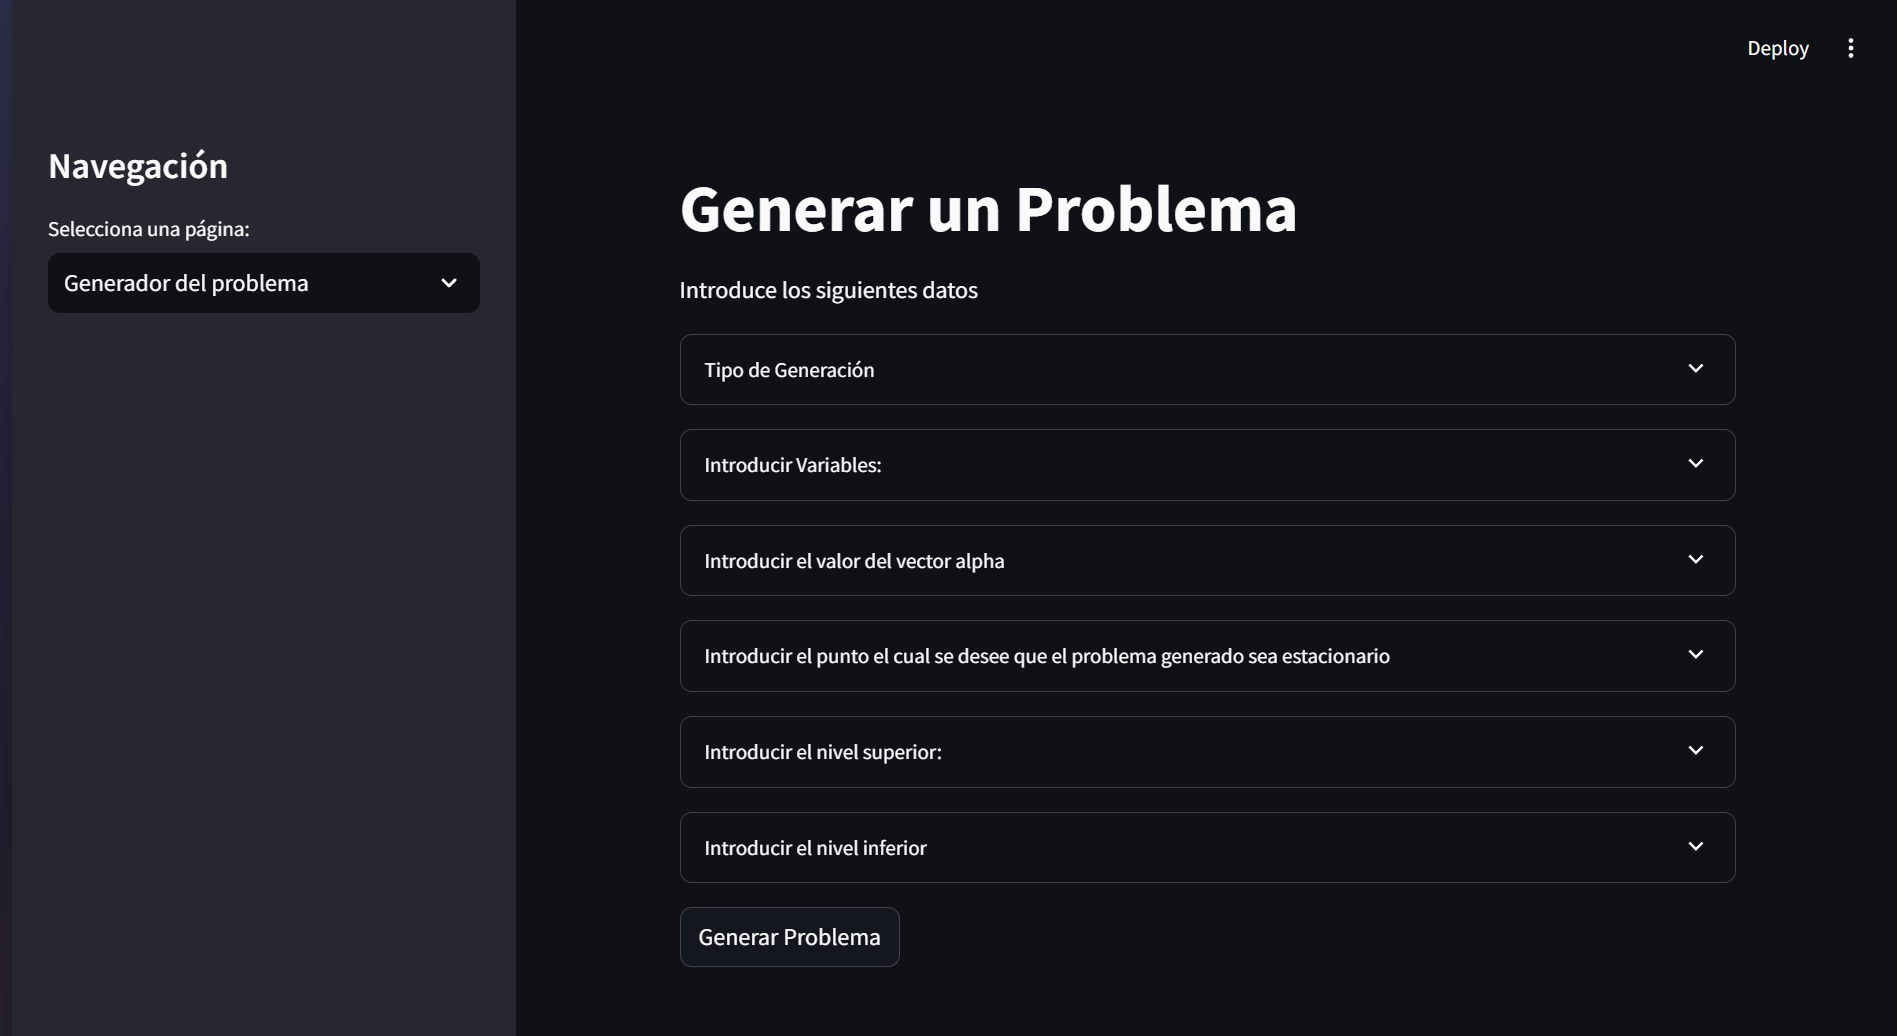
\includegraphics[width=\textwidth]{Graphics/front_streamlitpng.png}
    \caption{Pantalla principal de generación del problema}
    \label{fig:front_generator_page}
\end{figure}

\begin{figure}[H]
    \centering
    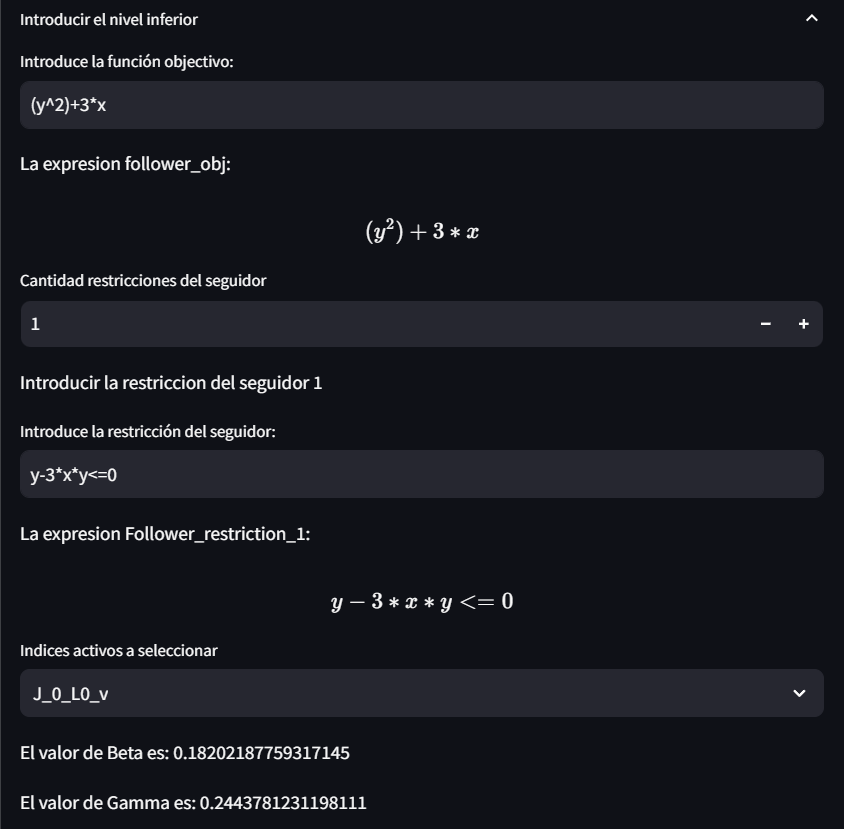
\includegraphics[width=\textwidth]{Graphics/Ejemplo_introducir_follower_rest.png}
    \caption{Ejemplo de generación de problema en punto Fuertemente Estacionario}
    \label{fig:example_strong_stationary_front_generator}
\end{figure}

	
	\include{Experimentación.tex}
	
	\chapter{Conclusiones}

%Explicar que se hizo
En esta tesis se desarrolló un algoritmo para la generación de problemas de optimización binivel con características específicas de estacionariedad en puntos determinados. El mismo tiene la capacidad de modificar problemas originales para garantizar la factibilidad y estacionariedad en puntos dados, aprovechando las capacidades del lenguaje de programación Julia, que destaca por su alto rendimiento computacional y sintaxis adaptada a problemas de optimización.

% Explicar como fue la experimentacion
La experimentación se llevó a cabo sobre tres categorías fundamentales de problemas: lineales, cuadráticos y no convexos. El proceso experimental comenzó con la obtención de puntos mínimos utilizando bibliotecas establecidas como BilevelJuMP y JuMP. Posteriormente, se generaron problemas estacionarios mediante la adición de componentes aleatorias a estos puntos para cada clase de problema definida.

% Que se comparó
Los problemas modificados fueron sometidos nuevamente a algoritmos tradicionales implementados en Julia para evaluar su efectividad frente a los puntos estacionarios generados. Se realizó un análisis comparativo destacando los casos más relevantes de cada categoría de puntos estacionarios, considerando la evaluación de la función objetivo del nivel superior en el punto donde se garantizó la estacionariedad, contrastándola con los resultados obtenidos por las bibliotecas convencionales.

% Recomendaciones
Como resultado de la investigación realizada, se han identificado varias líneas de trabajo futuro que permitirían expandir y mejorar los resultados obtenidos. En primer lugar, se recomienda ampliar el alcance de la experimentación numérica para incluir una mayor diversidad de problemas de optimización binivel. Esta expansión permitiría validar la robustez y versatilidad del algoritmo propuesto en diferentes contextos y escenarios de aplicación.

En segunda instancia, se sugiere profundizar en la investigación sobre la implementación del algoritmo desarrollado como criterio de parada en nuevos métodos de optimización binivel. Esta línea de investigación podría contribuir significativamente al desarrollo de algoritmos más eficientes y confiables, mejorando la capacidad de detectar y verificar puntos estacionarios durante el proceso de optimización.

Finalmente, se propone el desarrollo de una interfaz gráfica más intuitiva y funcional que facilite la generación automática de puntos según el tipo de estacionariedad requerida. Esta mejora en la usabilidad del software permitiría que usuarios con diferentes niveles de experiencia puedan aprovechar las capacidades del algoritmo de manera más efectiva, ampliando así su aplicabilidad práctica en diversos campos de estudio.

	%\chapter{Recomendaciones y Trabajo Futuro}

Como resultado de la investigación realizada, se han identificado varias líneas de trabajo futuro que permitirían expandir y mejorar los resultados obtenidos. En primer lugar, se recomienda ampliar el alcance de la experimentación numérica para incluir una mayor diversidad de problemas de optimización binivel. Esta expansión permitiría validar la robustez y versatilidad del algoritmo propuesto en diferentes contextos y escenarios de aplicación.

En segunda instancia, se sugiere profundizar en la investigación sobre la implementación del algoritmo desarrollado como criterio de parada en nuevos métodos de optimización binivel. Esta línea de investigación podría contribuir significativamente al desarrollo de algoritmos más eficientes y confiables, mejorando la capacidad de detectar y verificar puntos estacionarios durante el proceso de optimización.

Finalmente, se propone el desarrollo de una interfaz gráfica más intuitiva y funcional que facilite la generación automática de puntos según el tipo de estacionariedad requerida. Esta mejora en la usabilidad del software permitiría que usuarios con diferentes niveles de experiencia puedan aprovechar las capacidades del algoritmo de manera más efectiva, ampliando así su aplicabilidad práctica en diversos campos de estudio.
	
	\backmatter
	\printbibliography

\end{document}